% Layout adapted from the research memo shown in Lecture 1, sized for A4.
\documentclass[a4paper,10pt]{article}
\usepackage[margin=18mm,footskip=9mm]{geometry}
\usepackage{iftex}
\ifPDFTeX
  \usepackage[T1]{fontenc}
  \usepackage[utf8]{inputenc}
  \usepackage[scaled=0.96]{helvet}
  \renewcommand{\familydefault}{\sfdefault}
\else
  \usepackage{fontspec}
  \setmainfont{texgyreheros}[Extension=.otf,
    UprightFont=*-regular, BoldFont=*-bold,
    ItalicFont=*-italic, BoldItalicFont=*-bolditalic]
\fi
% For Chinese, set this switch true and compile with --engine xelatex.
\newif\ifChineseMemo
\ChineseMemofalse
\ifChineseMemo
  \ifPDFTeX
    \PackageError{finance-memo}{Chinese text requires XeLaTeX or LuaLaTeX}{}
  \else
    \usepackage[UTF8,fontset=fandol]{ctex}
    \renewcommand{\familydefault}{\sfdefault}
  \fi
\fi
\usepackage{booktabs,graphicx,xcolor,caption,xurl,fancyhdr}
\definecolor{MemoBlue}{HTML}{203E70}
\definecolor{MemoRule}{HTML}{B9C8DF}
\usepackage[colorlinks=true,linkcolor=MemoBlue,urlcolor=MemoBlue]{hyperref}
\captionsetup{font=small,labelfont=bf,skip=4pt}
\setlength{\parindent}{0pt}
\setlength{\parskip}{5pt}
\pagestyle{fancy}
\fancyhf{}
\renewcommand{\headrulewidth}{0pt}
\renewcommand{\footrulewidth}{0.3pt}

\newcommand{\ReportTitle}{MU FY2026 Q4: Neutral, target price \$1,102}
\newcommand{\ReportType}{EARNINGS UPDATE}
\newcommand{\ReportDate}{2026-11-15}
\newcommand{\DataDate}{2026-10-09 12:21:00 UTC}
\newcommand{\ReportScope}{Quarter ended 2026-09-03 (CY2026Q3); trigger filing 0000723125-26-000023}
\newcommand{\TeamName}{Semis Coverage (coursework)}
\newcommand{\DeskName}{AI semiconductor supply chain}
\newcommand{\ReportAuthor}{Coursework analyst (AI-assisted workflow)}
\newcommand{\Coverage}{NVDA, AMD, INTC, AVGO, MRVL, MU, AMAT}
\newcommand{\KeyFinding}{Revenue \$54.2bn (30.8\% q/q); target price \$1,102 vs last close \$1,035.84 (6.4\%).}
\fancyfoot[L]{\scriptsize\TeamName}
\fancyfoot[R]{\scriptsize\ReportType}

\begin{document}
\begin{minipage}[t]{0.70\textwidth}
\vspace{0pt}
{\small\ReportDate}\par\medskip
{\color{MemoBlue}\hrule height 0.5pt}\smallskip
{\large\ReportType}\par
{\LARGE\bfseries\ReportTitle}\par\medskip
\ReportScope
\end{minipage}\hfill
\begin{minipage}[t]{0.23\textwidth}
\vspace{0pt}\raggedleft
\colorbox{MemoBlue}{\parbox[c][19mm][c]{0.86\linewidth}{\centering\color{white}\bfseries\TeamName}}\par\medskip
\DeskName
\end{minipage}
\par\bigskip
{\color{MemoBlue}\hrule height 0.5pt}\medskip
{\large\KeyFinding}\par\bigskip

\begin{minipage}[t]{0.61\textwidth}
\vspace{0pt}\raggedright
\setlength{\parskip}{4pt}
\textbf{Summary}\par
See key points and full note below. Figures are generated by code from SEC filings; prose is AI-drafted and human-approved.
\end{minipage}\hfill
\begin{minipage}[t]{0.36\textwidth}
\vspace{0pt}\small
% Author these non-floating wrappers separately. Use \captionof{table/figure},
% then a description and \input/\includegraphics of generated content.
\IfFileExists{sections/tables.tex}{\captionof{table}{Key data, FY2026 Q4}\label{tab:key-data}
{\footnotesize Reported figures for the quarter ended 2026-09-03 (CY2026Q3) from SEC XBRL facts; NTM, DCF and target price are model outputs. US\$.\par}
\begin{tabular}{@{}lr@{}}
\toprule
Item & Value \\
\midrule
Revenue (quarter) & \$54.2bn \\
Revenue q/q & 30.8\% \\
Revenue y/y & 379.3\% \\
Gross margin & 86.8\% \\
Operating margin & 80.7\% \\
Free cash flow & \$32.9bn \\
\midrule
NTM revenue (model) & \$269.5bn \\
NTM EPS (model) & \$163.56 \\
DCF value / share & \$862.83 \\
Peer EV/Sales (median) & 15.1x \\
Last close & \$1,035.84 \\
Target price & \$1,102 \\
Upside & 6.4\% \\
Rating & Neutral \\
\bottomrule
\end{tabular}

}{
  \textbf{Key data}\par
  [Insert a compact checked table, including units and periods.]
}
\medskip
\IfFileExists{sections/figures.tex}{\captionof{figure}{Quarterly revenue, reported and forecast}\label{fig:revenue}
{\footnotesize Solid: reported (SEC XBRL, fiscal quarters). Hatched: model forecast from this case's assumptions. US\$ bn.\par}
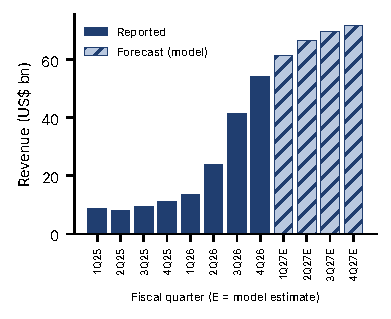
\includegraphics[width=\linewidth]{../../output/figures/MU-0000723125-26-000023/revenue.pdf}
}{
  \textbf{Supporting chart}\par
  [Insert a chart with readable labels, units, and a source note.]
}
\end{minipage}
\par\bigskip



*Fiscal quarter FY2026 Q4 / calendar quarter CY2026Q3, period ended 2026-09-03. Source filings: Form 10-K, accession 0000723125-26-000023, and the earnings release furnished earlier on Form 8-K, accession 0000723125-26-000018. Labels used below: "reported" means figures from the company's SEC XBRL data or derived from them by code, or company statements quoted from the filings; "our forecast" means outputs of our model assumptions; "our view" marks analyst judgment.*

\par\smallskip\textbf{\color{MemoBlue}Key points}\par

\begin{itemize}\setlength{\itemsep}{1pt}
\item \textbf{Reported:} revenue was \$54.2bn in FY2026 Q4, up 30.8\% sequentially and 379.3\% year on year, with a gross margin of 86.8\% and an operating margin of 80.7\%. FY2026 was a long year, and by our count from the reported period end dates the extra week fell in this quarter, which flatters both comparisons: “Fiscal 2026 contained 53 weeks and fiscal 2025 and 2024 each contained 52 weeks.”
\item \textbf{Guidance (reported):} for the first quarter of FY2027 management guides revenue of “\$61.5 billion ± \$1.5 billion” on both a GAAP and a non-GAAP basis (\$61.5bn at the midpoint). Gross margin guidance is “Approximately 85.95\%” on a GAAP basis and “Approximately 86.25\%” on a non-GAAP basis. Diluted EPS guidance is “\$37.84 ± \$1.00” on a GAAP basis and “\$38.15 ± \$1.00” on a non-GAAP basis.
\item \textbf{Our forecast:} FY2027Q1 revenue of \$61.5bn and EPS of \$37.50; next-twelve-month revenue of \$269.5bn and EPS of \$163.56.
\item \textbf{Valuation and rating:} our target price of \$1,102 implies 6.4\% upside to the 2026-10-08 close of \$1,035.84, inside the Neutral band. We rate the shares \textbf{Neutral}.
\item \textbf{Our view:} demand is strong and pricing is supported by new customer agreements, but the shares already discount much of the upswing, and our model assumes the memory cycle normalizes after FY2027 in the outer years of the DCF.
\end{itemize}

\par\smallskip\textbf{\color{MemoBlue}Results}\par

All figures in this section are reported (SEC XBRL data, with the fourth quarter derived by code as the fiscal year less the nine-month year-to-date).

\begin{itemize}\setlength{\itemsep}{1pt}
\item Revenue was \$54.2bn in FY2026 Q4, up 30.8\% quarter on quarter and 379.3\% year on year. Trailing-twelve-month revenue, which equals FY2026, was \$133.2bn.
\item Gross margin was 86.8\% and operating margin was 80.7\%. Net income was \$37.7bn.
\item Free cash flow (operating cash flow less capital expenditure) was \$32.9bn in the quarter.
\item Period length matters for comparisons: “Fiscal 2026 contained 53 weeks and fiscal 2025 and 2024 each contained 52 weeks.” By our calculation from the reported period end dates (the third quarter ended in May and the fourth on 2026-09-03), the fourth quarter carried the extra week, so the sequential and year-on-year growth rates above overstate the underlying run-rate change (our view; we have not computed a week-adjusted figure in code).
\item Management's characterisation of the year: ““Micron delivered record fiscal 2026 results, and we expect an even stronger fiscal 2027,” said Sanjay Mehrotra, Chairman and CEO of Micron Technology.”
\item Capital return: “On September 30, 2026, Micron’s Board of Directors declared a quarterly dividend of \$0.15 per share, payable in cash on October 29, 2026, to shareholders of record as of the close of business on October 14, 2026.”
\item Tax: “The change in our effective tax rate for 2026 as compared to 2025 was primarily due to the 15\% minimum tax Pillar Two Model Rules (“Pillar Two”).”
\end{itemize}

\par\smallskip\textbf{\color{MemoBlue}Guidance and outlook}\par

Company guidance (reported in the earnings release furnished on Form 8-K). “The following table presents Micron’s guidance for the first quarter of 2027:”

\par\smallskip{\small\begin{tabular}{p{\dimexpr 0.333\linewidth-2\tabcolsep}p{\dimexpr 0.333\linewidth-2\tabcolsep}p{\dimexpr 0.333\linewidth-2\tabcolsep}}
\toprule
\textbf{Item and basis} & \textbf{Company guidance (verbatim)} & \textbf{Code value (rounded)} \\
\midrule
Revenue, GAAP and non-GAAP & “\$61.5 billion ± \$1.5 billion” & \$61.5bn midpoint \\
Gross margin, GAAP & “Approximately 85.95\%” & 86.0\% \\
Gross margin, non-GAAP & “Approximately 86.25\%” & 86.2\% \\
Operating expenses, GAAP & “Approximately \$2.31 billion” & \$2.3bn \\
Operating expenses, non-GAAP & “Approximately \$2.06 billion” & \$2.1bn \\
Diluted EPS, GAAP & “\$37.84 ± \$1.00” & \$37.84 midpoint \\
Diluted EPS, non-GAAP & “\$38.15 ± \$1.00” & \$38.15 midpoint \\
\bottomrule
\end{tabular}}\par\smallskip

The verbatim quotes are authoritative for the precision of the guidance. Code stores each guided value at the quoted precision, but its display rounds percentages to one decimal place and amounts in billions to one decimal place, so the code column is shorter than the quotes; for the non-GAAP gross margin the display rounds the quoted figure down. Our model uses the GAAP guidance.

Demand and pricing context from the 10-K:

\begin{itemize}\setlength{\itemsep}{1pt}
\item “AI-driven memory and storage demand growth is outpacing industry supply.”
\item “The AI-driven growth in the data center has accelerated demand for memory and storage at a rate greater than our ability and the industry’s ability to increase supply.”
\item “In the third and fourth quarters of 2026, we entered into, and expect to continue to enter into, strategic customer agreements.”
\item “We expect gross margins from our strategic customer agreements with price bands, even at floor pricing levels, to yield gross margins meaningfully above our peak quarterly margins in any past cycle.”
\end{itemize}

\textbf{Our view:} the guidance points to further sequential growth and a gross margin close to the FY2026 Q4 level. Supply constraints limit volume growth, so we think pricing and the strategic customer agreements drive most of the near-term upside. The price bands support margins but also cap pricing upside.

\par\smallskip\textbf{\color{MemoBlue}Model and valuation}\par

\textbf{Our forecast (model assumptions, not company guidance):}

\begin{itemize}\setlength{\itemsep}{1pt}
\item FY2027Q1 revenue of \$61.5bn is anchored on the guidance midpoint of \$61.5bn. Sequential growth then slows through the rest of FY2027 (our view).
\item Gross margin is held flat at the GAAP guidance of “Approximately 85.95\%” for all four forecast quarters. Operating expenses are set at the guided GAAP ratio to revenue (“Approximately \$2.31 billion” on the revenue midpoint), and the tax rate is the FY2026 effective rate, which reflects Pillar Two (“The change in our effective tax rate for 2026 as compared to 2025 was primarily due to the 15\% minimum tax Pillar Two Model Rules (“Pillar Two”).”).
\item FY2027Q1 EPS of \$37.50 sits just below the GAAP EPS guidance midpoint of \$37.84, mainly because the model excludes interest income.
\item Next-twelve-month revenue is \$269.5bn and EPS is \$163.56.
\end{itemize}

\textbf{Valuation (code output from our inputs):}

\begin{itemize}\setlength{\itemsep}{1pt}
\item The discounted cash flow value is \$862.83 per share. The terminal value is 56\% of enterprise value. The DCF assumes a cycle peak followed by revenue normalization and declining free-cash-flow margins in the outer years (our view).
\item The peer cross-check uses a median EV/Sales multiple of 15.1x for a group of fab-owning and wafer-fab-equipment companies. None of them is a memory maker, so we give this method the minority weight and the DCF the majority weight.
\item Net cash is \$68.3bn: cash and cash equivalents plus short- and long-term marketable investments, less total debt (code output). Both valuation methods add this net cash to reach equity value per share.
\item The blended target price is \textbf{\$1,102}, 6.4\% above the 2026-10-08 close of \$1,035.84. That is below the Outperform threshold of +15\% and above the Underperform threshold of -10\%, so the rating is \textbf{Neutral}.
\end{itemize}

\textbf{Valuation caveat (our view, analyst judgment):} refundable customer deposits received under the strategic customer agreements are recorded as noncurrent customer contract liabilities. We treat them as operating liabilities and do not deduct them as debt in net cash. The 10-K classifies them as contract liabilities rather than debt, and a deposit is returned only if the customer meets its minimum purchase commitments. However, the cash received sits inside reported cash, the 10-K says nearly all of the deposits are scheduled to be repaid between 2029 and 2031, and our free-cash-flow path does not include that repayment. Treating the deposits as debt-like would therefore lower our valuation modestly; we have not computed that alternative in code.

\par\smallskip\textbf{\color{MemoBlue}Risks}\par

\begin{itemize}\setlength{\itemsep}{1pt}
\item \textbf{Cycle risk (our view):} memory pricing has historically mean-reverted after supply-constrained peaks. If supply catches up sooner than we model, revenue and margins could fall faster than in our DCF. If tightness lasts longer, our outer-year normalization is too conservative.
\item \textbf{Trade and export controls:} “International trade disputes, geopolitical tensions, and military conflicts have led, and continue to lead, to new and increasing export restrictions, trade barriers, tariffs, and other measures, as well as retaliatory actions, that can increase our manufacturing costs, make our products less competitive, reduce demand for our products, limit our ability to sell to certain customers or markets, limit our ability to procure or increase our costs for components or raw materials, impede or slow the movement of our goods across borders, impede our ability to perform R\&D activities, or otherwise restrict our ability to conduct operations.” We do not model this risk separately.
\item \textbf{Comparability:} the extra week in FY2026 Q4 (“Fiscal 2026 contained 53 weeks and fiscal 2025 and 2024 each contained 52 weeks.”) distorts growth rates and the trailing base used for the EV/Sales cross-check.
\item \textbf{Valuation inputs:} the discount rate and terminal assumptions are analyst judgments. The snapshot has no market-implied inputs to calibrate them. The peer group contains no memory makers. The treatment of customer deposits described above is also a judgment that favours the shares.
\item \textbf{Data gaps:} the 10-K XBRL does not tag a fourth-quarter diluted share count or diluted EPS. The share count used in the model is the latest tagged quarterly figure.
\end{itemize}

\par\smallskip\textbf{\color{MemoBlue}Disclosures}\par

\begin{itemize}\setlength{\itemsep}{1pt}
\item For coursework demonstration only; not investment advice.
\item Data sources (SEC EDGAR):
\item The Form 10-K for the fiscal year ended 2026-09-03, accession 0000723125-26-000023. Its SEC acceptance time sets the information cutoff of 2026-10-09 12:21 UTC.
\item The earnings release, furnished separately on Form 8-K, accession 0000723125-26-000018, in September 2026, before the 10-K. It is the source of the guidance, the chief executive's statement and the dividend announcement quoted above.
\item SEC XBRL company facts as of the cutoff.
\item Share price is the last close before the cutoff, \$1,035.84 on 2026-10-08. No information after the cutoff was used.
\item Rating definitions: Outperform means upside to the target price of +15\% or more; Underperform means upside of -10\% or less; otherwise Neutral.
\item Figures are generated by code from SEC XBRL data and are unaudited by the author. Forecasts and valuation inputs are analyst assumptions, and statements marked "our view" are analyst judgment.
\end{itemize}

\par\smallskip\textbf{\color{MemoBlue}Open review findings}\par

The independent critics recorded these findings. They are minor, so they did not block acceptance, and the note above was not changed for them. Readers should take them into account.

\begin{itemize}\setlength{\itemsep}{1pt}
\item asm-004 (minor): Pillar Two noncurrent income taxes payable (\$9.82B) is not addressed in the net cash or FCF rationale
\item asm-005 (minor): The rating depends on the DCF/EV-Sales weight, and the note does not show the relative-value leg
\item cmp-004 (minor): Disclosures list the share price under 'Data sources (SEC EDGAR)', but the price does not come from SEC EDGAR
\item prov-005 (minor): Customer-deposit caveat paraphrases the 10-K more strongly than the source and is not quote-backed
\end{itemize}

\par\vfill

{\color{MemoRule}\hrule height 0.4pt}\medskip
\begin{minipage}[t]{0.36\textwidth}
\vspace{0pt}\small
\setlength{\parskip}{3pt}
\textbf{PREPARED BY}\par\ReportAuthor\par\TeamName\par
\medskip\textbf{COVERAGE}\par\Coverage
\end{minipage}\hfill
\begin{minipage}[t]{0.60\textwidth}
\vspace{0pt}\footnotesize
\setlength{\parskip}{3pt}
\textbf{Sources and dates.} Data as of \DataDate.
SEC EDGAR filings accepted at or before 2026-10-09T12:21:00Z (trigger 0000723125-26-000023); last close \$1,035.84 on the cutoff date from the Yahoo chart endpoint. Case files: cases/MU-0000723125-26-000023.

\textbf{Checks.} Numerical and provenance gates passed; two consecutive clean reviews by three independent critics (round 2); approved by Repository owner (kuostudy31-bot); executed by Claude under the owner's delegation of 2026-11-14 on 2026-11-15.

\textbf{Preparation.} Claude Code agent team (orchestrator, generator and critic leads, eight specialists) under a Python controller; for coursework demonstration only, not investment advice.
\end{minipage}
\end{document}
